\section{Design}
\label{sec:design}

%%\begin{figure}[t]
%%    \centering
%%    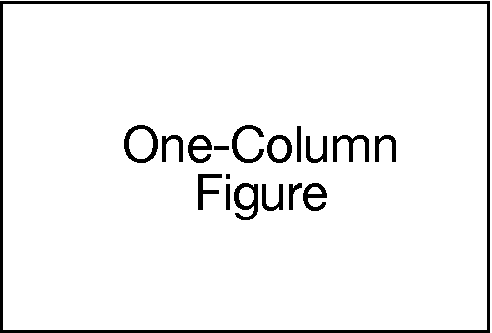
\includegraphics{diagrams/template.pdf}
%%    %
%%    \caption{High-level architecture.}
%%    %
%%    \label{fig:architecture}
%%\end{figure}

\parhead{Trusted function runtime.}
%
For \SystemName's function runtime, we will extend \emph{Project Oak},\footnote{
\url{https://github.com/project-oak/oak}
%\url{https://nordprojects.co/projects/oak/}
}
an open-source framework for processing private data within a TEE\@.
%
The central component of Project Oak is the \emph{Oak Functions} platform (see
Figure~\ref{fig:oak}), which executes each function in a confidential VM with a
custom, minimal operating system kernel designed to execute only a single
process.
%
\begin{figure}
    \centering
    \includegraphics[page = 3, width=0.48\textwidth]{diagrams/slides.pdf}
    %
    \caption{Oak and DICE architecture.
    %
    In the DICE model, each software layer loads and measures the next layer,
    generates an ephemeral key pair for the layer, and issues the layer a
    certificate endorsing its measurement and public key.
    %
    Oak uses AMD's trusted hardware as the root of trust.
    %
    % In total, Oak's implementation of DICE results in a certificate chain, rooted
    %in the AMD trusted hardware, that attests the entire workload.
    }
    \label{fig:oak}
\end{figure}
%
The function runs in a secure WebAssembly (Wasm) runtime sandbox, preventing
the process from leaking any sensitive client data.
%
Additionally, Oak uses the DICE~\cite{24-misc-dice} architecture for measured
boot to extend AMD SEV-SNP's attestation from the initial state of the VM
to the entire VM workload.
%
We will modify the Oak kernel with cryptographic support to transparently
manage keys and encrypt I/O\@.



\parhead{Key management.}
%
In previous research, each function replica would attest to a trusted key
server to obtain a shared key pair.
%
To eliminate this central, trusted dependency, \SystemName
uses decentralized key management with proxy re-encryption.
%
\begin{figure}
    \centering
    \includegraphics[page = 4, width=0.48\textwidth]{diagrams/slides.pdf}
    %
    \caption{\SystemName architecture.}
    %
    \label{fig:arch}
\end{figure}
%
As Figure~\ref{fig:arch} illustrates, the first instance of a function
generates a key pair and registers the public key in an untrusted registry,
along with an attestation report that proves the key was generated in an Oak
TEE\@.
%
%As shown in Figure~\ref{fig:arch},
%the first instance of a function generates a key pair and registers the
%public key in an untrusted registry with an attestation report from an Oak
%TEE\@.
%attestation report that verifies the key was generated in an Oak TEE\@.
%
When a new replica is launched, the replica registers its own public key,
prompting the original instance to generate a re-encryption key.
%
%This enables any instance to encrypt messages for the original key pair,
%allowing independent scaling.
%
As a result, each function can encrypt messages for the original downstream
instance's public key, remaining independent of that function's scaling.



%%
%In previous research, to ensure each function replica used the same key pair,
%each replica would attest to a trusted key server, which then provided the
%correct key pair based on the replica's attestation measurement.
%%
%To remove this reliance on centralized, trusted infrastructure, \SystemName
%employs a decentralized key management system using proxy re-encryption.
%%
%\begin{wrapfigure}{l}{0.5\textwidth}
%    \centering
%    \includegraphics[page = 4, width=0.48\textwidth]{diagrams/slides.pdf}
%    %
%    \caption{\SystemName architecture.}
%    %
%    \label{fig:arch}
%\end{wrapfigure}
%%
%As Figure~\ref{fig:arch} illustrates, the initial instance of the function
%generates a key pair and registers the public key in an untrusted registry,
%along with an attestation report that verifies the key was generated in an Oak
%TEE\@.
%%
%When the FaaS platform launches a new replica of the function, the replica
%generates and registers its own public key.
%%
%This triggers the FaaS platform to request the initial function instance to
%produce a re-encryption key for the new replica.
%%
%As a result, each function can encrypt messages for the original instance’s
%public key, remaining independent of the function's scaling.


\parhead{Control flow integrity.}
%
Beyond encrypting function I/O, \SystemName must ensure the integrity
of the sequence of functions.
%
%Guaranteeing this property is challenging, as a function chain can span multiple
%organizations, and an organization may be unaware of its functions position in
%the chain.
%
\SystemName approaches this challenge in two ways.
%
First, we extend the Oak runtime to include a cryptographically binding record
of provenance: each function extends a path signature by signing over its
current link.
%
The last function then posts this provenance record to an untrusted log that
any organization can monitor and audit.
%
Additionally, if an organization knows a flow graph for the function chain (or
some subset thereof),  Oak will locally verify that the received event and the
function's subsequent output conform to the graph.


\parhead{Optimization.}
%
\SystemName relies on certificate chains both for attestation and provenance.
%
To reduce bandwidth and storage costs, \SystemName can compress the chains
using an aggregate signature
scheme~\cite{03-eurocrypt-aggregate_signatures_bilinear_maps}.
%
In an \emph{aggregate signature},
each private key $sk_i$ signs a \emph{distinct} message $m_i$ to form signature
$\sigma_i$, and any party can compress the $\sigma_i$ into a single,
small aggregate signature $\sigma^*$.  
%
The aggregate signature convinces a verifier that each signer signed their
respective message.

%%\begin{table}[t!]
%%    \small
%%    \caption{Time (s) to Re-encrypt a Bucket of Size 1G}
%%    \label{tab:enclave-overhead}
%%    \centering
%%    \begin{tabular*}{0.48\textwidth}{|r|@{\extracolsep{\fill}}r|r|}
%%        \hline
%%        \textbf{Environment}  &\textbf{Akeso}  &\textbf{Strawman}  \\
%%        \hline
%%        \textbf{Confidential VM}    &47.231  	 &118.239  \\             
%%        \textbf{Non Confidential VM}        &44.907	    &109.366 \\            
%%        \hline 
%%    \end{tabular*}
%%\end{table}

\textbf{adwait}

There are a number of open source projects for various parts of the project that we will be extending.

\subsection{Function Runtime}
We performed all development and testing on an AMD-SEV SNP machine, to later take advantage of Trusted Execution Environment features.
We have not yet enabled these features in the course of development.
We ported an open source proxy re-encryption library from C to Rust in order to be callable from within the later boot stages of the Oak Restricted Kernel.
The kernel extension itself is still a work in progress.
There is a lot to sort through to determine where exactly in the boot stages would be the best place to perform re-encryption and decryption
to be able to work with the data.

\subsection{FaaS Orchestration}
Function as a Service paradigms are implemented differently by different platforms.
Amazon Lambda, Google Cloud Functions, and Azure Functions are all well-known and closed source, all with (presumably) completely different architectures.

The open source FaaS landscape is no more homogenous than its corporate counterpart.
Additionally, some are partially open source, with certain paywalled features, and others use deprecated dependencies which makes setup a non-trivial problem.
This was a major hurdle for development, and battling the idiosyncracies of these FaaS frameworks accounts for much of the progress (or lack thereof) made on this project.

\subsubsection{Firecracker}
Firecracker is partially open source, and disbatches requests to networks of MicroVMs.
Since it doesn't support custom kernels out of the box, and a lot of the code is written with MicroVM specific APIs, extending this project to accomodate the Oak Restricted Kernel for SAMBA would amount to basically a full rewrite.

\subsubsection{OpenFaaS}
OpenFaaS, perhaps misleadingly, is not fully open source.
Components such as the load balancer that creates function replicas are only availible as binaries, and therefore the modifications that we need to make are not possible with OpenFaaS.

\subsubsection{OpenWhisk}
OpenWhisk is fully open source, and is used in a variety of recent papers. That said, the repository seems barely maintained in 2024, and older versions of Java (Java 8), Docker, and Ubuntu may be required to cohesiveliy run it.
Investigations to that effect are another significant contributor to delay in this project.
We anticipate continuing efforts, potentially of a known working fork from a researcher who has used OpenWhisk successfully in recent years.
Also, I will re-double my efforts following and modifying few-yearold open source documentation to get development up and running, by emulating all dependencies as closely as possible.

\subsubsection{Open Function}
Open Function is another open source function orchestrator, which we will look into as an implementation option.
